\begin{frame}\frametitle{Hoe ziet een rooster eruit?}
	\begin{columns}[T]
	    \begin{column}{.4\textwidth}
			\begin{itemize}
		        \item Activiteiten
		        \begin{itemize}
		            \item Stoelen vervangen
		            \item Graffiti verwijderen      
		        \end{itemize}
		        \item Resources
	            \begin{itemize}
	                \item Monteurs
	                \item Schoonmakers
	                \item Werkplaatsen
	            \end{itemize}
		    \end{itemize}
	    \end{column}
	    \begin{column}{.5\textwidth}
	    	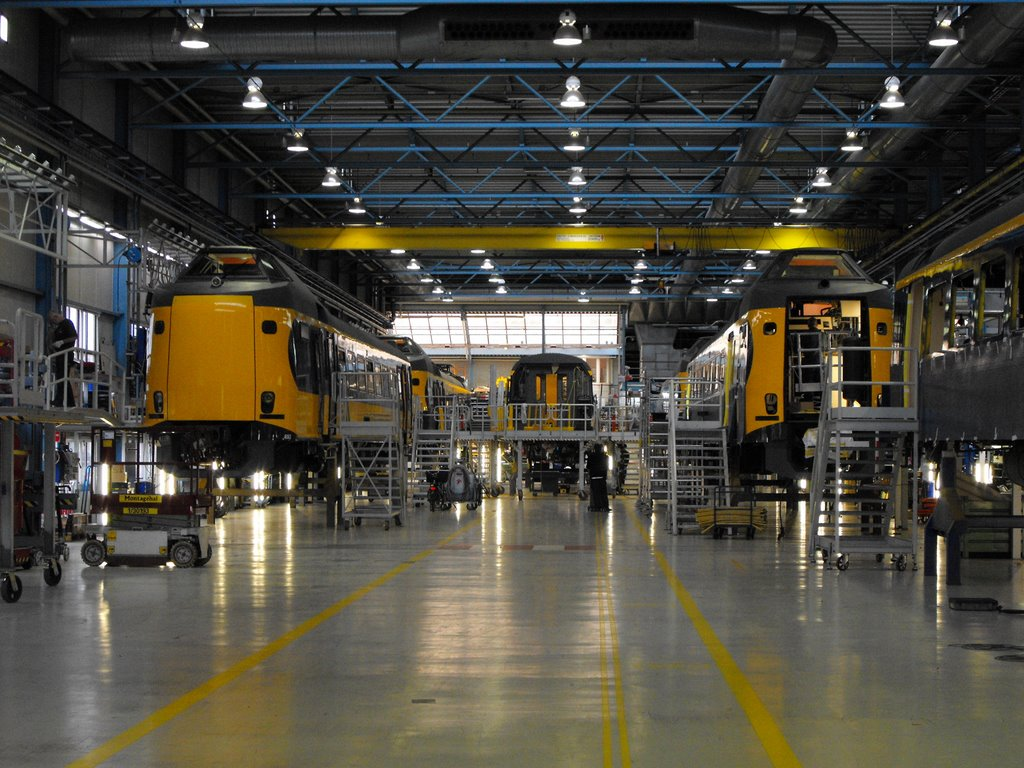
\includegraphics[width=4.5cm]{images/werkplaats.jpg}
	    \end{column}
  	\end{columns}
    \begin{itemize}
        \item Constraints
        \begin{itemize}
        	\item Capaciteit resources
            \item Deadlines van activiteiten
            \item Activiteit mag pas starten na afronden andere activiteit 
        \end{itemize}
    \end{itemize}
\end{frame}
